%Empieza configuracion de capitulo
\setstretch{1.0}
\titleformat{\chapter}[block]{\Large\bfseries}{CHAPTER \Huge\thechapter\vspace{25 pt}}{0 pt}{\\\fontsize{26}{36}\selectfont}
\titlespacing{\chapter}{0 pt}{30 pt}{50 pt}[0 pt]
\titleformat{\section}{\Large\bfseries}{\thesection}{0 pt}{\hspace{30 pt}}
\titleformat{\subsection}{\large\bfseries}{\thesubsection}{0 pt}{\hspace{30 pt}}
\pagestyle{fancy}
\fancyhead[LO,LE]{\footnotesize\textit{\leftmark}}
\fancyhead[RO,RE]{\thepage}
\fancyfoot[CO,CE]{}
%Termina configuracion de capitulo

\chapter{Promela Model and LTL Properties} %Cambia al nombre de tu capitulo
\setstretch{1.5} %Regresa el interlineado a 1.5

\lstset{
language=Promela,
numbers=left,
numberstyle=\small,
frame=tb,
columns=fullflexible,
showstringspaces=false,
framexleftmargin=15pt
}

\normalsize
\noindent
The purpose of this section is to introduce the model proposed for specifying the rule-based plans and to expand on the LTL properties to verify the model.  
\section{Rule-based Plans Model}
\subsection{Overview}
\noindent
The key element to model is the specification of the rule-based plans. For that purpose, we declared a number of user-defined data types (i.e. typedef data structures), which are shown in a typedef diagram below in figure \ref{TypeDef_Diagram}. \\

\begin{figure}[H]
\centering
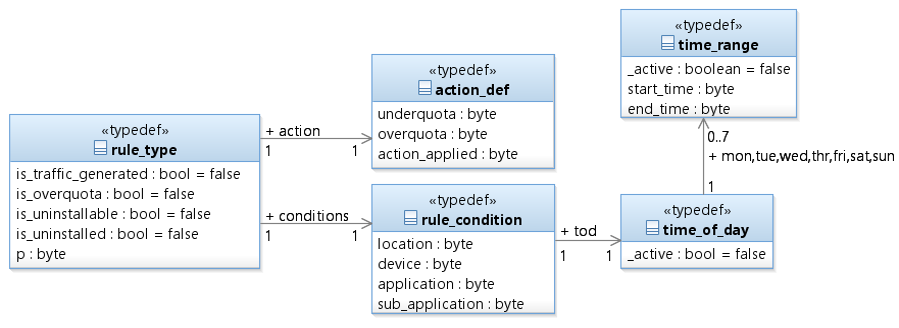
\includegraphics[width=1\textwidth]{image/TypeDef_Diagram}
\caption{Typedef diagram}
\label{TypeDef_Diagram}
\end{figure}
\subsubsection{Rule Type}
\noindent
This data type allows us to specify a rule with its attributes described in table \ref{ruletype_attributes} below. Additionally, each rule, declares one \emph{action{\_}def} variable and one \emph{rule{\_}conditions} variable, described respectively in tables \ref{actiondef_attributes} and \ref{ruleconditions_attributes} below. \\

\begin{table}[H]
\begin{center}
\scalebox{0.8}{	
\begin{tabular}{| l || p{2cm} | p{8cm} | p{4.5cm} |}
\hline
\textbf{Attribute} & \textbf{Type} & \textbf{Description} & \textbf{Example} \\
 \hline \hline
\emph{is{\_}generated{\_}traffic} & bool & If traffic is generated for this particular rule, \emph{is{\_}generated{\_}traffic} attribute is set to true. & true | false   \\ \hline
\emph{is{\_}overquota} & bool & If this attribute is set to true, the current state of the rule is \emph{overquota}. If it is set to false, then it is \emph{underquota}. & true | false   \\ \hline
\emph{is{\_}uninstallable} & bool & If this is set to true, this rule will eventually be uninstalled when its quota is reached. & true | false   \\ \hline
\emph{uninstalled} & bool & If this is set to true, this rule has been uninstalled and it is no longer active. & true | false   \\ \hline
\emph{p} & byte & \emph{p} stands for the \emph{priority} of the rule. Valid values are from 0 to 255. & 5   \\ \hline

\end{tabular}}
\end{center}
\caption{\emph{Rule{\_}Type} Attribute definitions. }
\label{ruletype_attributes}
\end{table}

\subsubsection{Action Def}
\noindent
This data type allows us to specify the actions to be applied for each state of the rule. 

\begin{table}[H]
\begin{center}
\scalebox{0.8}{	
\begin{tabular}{| l || p{2cm} | p{8cm} | p{4.5cm} |}
\hline
\textbf{Attribute} & \textbf{Type} & \textbf{Description} & \textbf{Example} \\
 \hline \hline
\emph{underquota} & byte & The action to be applied when the rule is in the underquota state. & \makecell[l]{0:block \\ 1:allow}   \\ \hline
\emph{overquota} & byte & The action to be applied when the rule is in the overquota state. & \makecell[l]{0:block \\ 1:allow}   \\ \hline
\emph{action{\_}applied} & byte & To store the current action applied. & \makecell[l]{0:block \\ 1:allow}   \\ \hline
\end{tabular}}
\end{center}
\caption{\emph{Action{\_}Def} Attribute definitions. }
\label{actiondef_attributes}
\end{table}

\subsubsection{Rule Conditions}
\noindent
This data type allows us to specify the conditions for the rule described in table \ref{ruleconditions_attributes} below. Additionally, each rule condition, declares one \emph{time{\_}of{\_}date} variable for specifying the different time conditions for each day. Whenever the conditions are met, the actions specified are performed. \\

\begin{table}[H]
\begin{center}
\scalebox{0.8}{	
\begin{tabular}{| l || p{2cm} | p{8cm} | p{4.5cm} |}
\hline
\textbf{Attribute} & \textbf{Type} & \textbf{Description} & \textbf{Example} \\
 \hline \hline
\emph{location} & byte & The location condition for applying the rule actions. & \makecell[l]{0:local \\ 1:roaming}   \\ \hline
\emph{device} & byte & The device condition for applying the rule actions. & \makecell[l]{0:Mobile \\ 1:Tablet \\ 2:Smart TV}   \\ \hline
\emph{application} & byte & The application condition for applying the rule actions. & \makecell[l]{0:Social Networks \\ 1:Video Streaming}   \\ \hline
\emph{subapplication} & byte & The subapplication condition for applying the rule actions. & \makecell[l]{For Social Networks\\0:Facebook \\ 1:Twitter \\ 2:Instagram}   \\ \hline
\end{tabular}}
\end{center}
\caption{\emph{Rule{\_}Conditions} Attribute definitions. }
\label{ruleconditions_attributes}
\end{table}

\subsubsection{Time of Day and Time Ranges conditions}
\noindent
As shown in table \ref{tod_attributes} below, the time{\_}of{\_}day data type allows us to specify the time conditions for each day. 

\begin{table}[H]
\begin{center}
\scalebox{0.8}{	
\begin{tabular}{| l || p{2cm} | p{8cm} | p{4.5cm} |}
\hline
\textbf{Attribute} & \textbf{Type} & \textbf{Description} & \textbf{Example} \\
 \hline \hline
\emph{{\_}active} & bool & Determines whether or not there is a time condition defined. & true | false   \\ \hline
\makecell[l]{\emph{mon, tue, wed,} \\ \emph{thr, fri, sat, sun}} & time{\_}range & Time conditions for each day. & See table \ref{tr_attributes} below \\ \hline
\end{tabular}}
\end{center}
\caption{\emph{Time{\_}of{\_}day} Attribute definitions. }
\label{tod_attributes}
\end{table}
As shown below in table \ref{tr_attributes}, each time-day condition compromises a start time and end time. 
\begin{table}[H]
\begin{center}
\scalebox{0.8}{	
\begin{tabular}{| l || p{2cm} | p{8cm} | p{4.5cm} |}
\hline
\textbf{Attribute} & \textbf{Type} & \textbf{Description} & \textbf{Example} \\
 \hline \hline
\emph{{\_}active} & bool & Determines whether or not there is a time condition defined for this particular day. & true | false   \\ \hline
\emph{start{\_}time} & byte & Start time condition. & 08  \\ \hline
\emph{end{\_}time} & byte & End time condition. & 20  \\ \hline
\end{tabular}}
\end{center}
\caption{\emph{Time Range} Attribute definitions. }
\label{tr_attributes}
\end{table}

\subsection{Process Definition}
\noindent
Two processes, explained in detailed below, have been defined to model rule-based plans: Priority Checker and OverQuota.

\subsubsection{Priority Checker}
\noindent
The Priority Checker process randomly chooses two rules, and executes the rule with higher priority. Listing \ref{lsl_prioritychecker} below, shows an informal description of the PriorityChecker process. \\

The process starts in line 2, by randomly selecting two-rule indexes ``x'' and ``y'', and initializing a bool local variable local\_overquota to store whether or not the rule is overquota. \\

In line 10 below, the PriorityChecker process verifies that the two random indexes are different and  that the rule with the index ``x'' has not been uninstalled yet by the OverQuota process. If the verification passes, then the rule ``x'' is flagged with the traffic generated attribute (line 12). If not, no traffic is generated for that rule (line 28). \\

From line 11 to 24 below, the PriorityChecker process atomically checks if the conditions of the rules ``x'' and ``y'' are different, or if rule ``x'' has a higher priority assigned. If any of those scenarios are met, then the underquota action configured for rule ``x'' is applied and the process waits for the overquota state (lines 15 and 20). If not, no action is applied for rule ``x''. \\

Finally, from line 25 to 28 below, the overquota action configured for rule ``x'' is applied if the local overquota is true. If not, no action is applied for rule ``x''. 

\singlespacing
\begin{lstlisting}[caption=PriorityChecker high-level algorithm,
  label=lsl_prioritychecker]
  proctype PriorityChecker () {
    // Pick two random rules x and y.
    int x;
    select (x : 0 .. (num_R-1)); 
    int y;
    select (y : 0 .. (num_R-1)); 
  
    bool local_overquota=false;

    if (x !=y and !Rules[x].is_uninstalled) then 
      atomic{
        Rules[x].is_traffic_generated = true;  
        if (conditions of Rules[x] != conditions of Rules[y]) then
          Rules[x].action.action_applied = (Rules[x].action.underquota);
          (Rules[x].is_overquota == true);
          local_overquota = true;
        else
          if (Rules[x].p > Rules[y].p) then 
            Rules[x].action.action_applied = (Rules[x].action.underquota);
            (Rules[x].is_overquota == true);
            local_overquota = true;
          else
            Rules[x].action.action_applied=NO_ACTION;      
      }
      if local_overquota then 
        Rules[x].action.action_applied = (Rules[x].action.overquota);
      else
        Rules[x].action.action_applied=NO_ACTION; 
    else
      Rules[x].is_traffic_generated = false;  
  }    	
\end{lstlisting}
\doublespacing

Refer to the Appendix A to review the Promela Code for the PriorityChecker process, detailed in Listing  \ref{lsl_prioritychecker_r}. 

\subsubsection{OverQuota}
\noindent
The OverQuota process iterates through the array of defined rules, and change each state from underquota to overquota over time. Additionally, if the rule is flagged as uninstallable, the is\_uninstallable attribute is set to true as well. \\

Refer to the Appendix A to review the Promela Code for the OverQuota process, detailed in Listing  \ref{lsl_overquota_r}. 
\subsection{Example of rule-based plans}
\noindent
A mobile operator, would like to offer free local facebook to its subscribers. The following Promela code would represent that rule in our model. 


\singlespacing
\begin{lstlisting}[caption=Free Facebook Rule.,
  label=fb_listing]
   rule_type freeFB
   freeFB.conditions.application = 0; //Facebook
   freeFB.conditions.location = 0; //local
   freeFB.action.underquota = 1;
   freeFB.action.overquota = 1;
   freeFB.p = 1;
\end{lstlisting}
\doublespacing

Additionally, the same mobile operator may also need to offer a limited amount of bytes that could be consumed in a monthly basis. As shown in the listing \ref{nav_listing} below, traffic is allowed (1) for any type of traffic generated when underquota. Once overquota, the action is blocked (0). 255 is used as the wildcard for specifying any application and any location. 

\singlespacing
\begin{lstlisting}[caption=Free Navigation Rule.,
  label=nav_listing]
   rule_type navRule
   navRule.conditions.application = 255;
   navRule.conditions.location = 255;
   navRule.action.underquota = 1;
   navRule.action.overquota = 0;
   navRule.p = 0;
\end{lstlisting}
\doublespacing

\section{LTL Properties}
\subsection{Macros Definitions}
\noindent
As seen before, Linear-Temporal-Logic formulas will be used to verify if the model satisfies the specification. If it is not satisfied, the system requirements, may not be well defined.\\

Listing \ref{macros_listing} below, enumerates the macros we have defined for each rule to be used in the LTL formulas to prove the predefined System properties. 

\singlespacing
\begin{lstlisting}[caption=Macros for each rule,
  label=macros_listing]
  #define generated_rule_X (Rules[X].is_traffic_generated)
  #define allowed_rule_X (Rules[X].action.actionApplied==ALLOWED_ACTION)
  #define blocked_rule_X (Rules[X].action.actionApplied==BLOCKED_ACTION)
  #define overquota_rule_X (Rules[X].is_overquota)
\end{lstlisting} \bigskip
\doublespacing

A further description of each macro is presented in table \ref{macros} below.

\begin{table}[H]
\begin{center}
\scalebox{0.8}{	
\begin{tabular}{| l || p{7cm} | p{7.1cm} |}
\hline
\textbf{Macro} & \textbf{Description} & \textbf{Expression} \\
 \hline \hline
\emph{generated{\_}rule{\_}$\{$index$\}$} & Whenever the Priority Checker process generates traffic for this particular rule, this macro will be evaluated to true. & Rules[$\{$index$\}$].is{\_}traffic{\_}generated\\ \hline
\emph{allowed{\_}rule{\_}$\{$index$\}$} & Whenever the Priority Checker process applies the allowed action ("1"), this macro evaluates to true. & Rules[$\{$index$\}$].action.action{\_}applied== ALLOWED{\_}ACTION\\ \hline
\emph{blocked{\_}rule{\_}$\{$index$\}$} & Whenever the Priority Checker process applies the blocked action ("0"), this macro evaluates to true. & Rules[$\{$index$\}$].action.action{\_}applied== BLOCKED{\_}ACTION\\ \hline
\emph{overquota{\_}rule{\_}$\{$index$\}$} & Whenever the Overquota process sets the current state of the rule as overquota, this macro evaluates to true. & Rules[$\{$index$\}$].is{\_}overquota\\ \hline
\end{tabular}}
\end{center}
\caption{Macros Definitions}
\label{macros}
\end{table}

\subsection{Properties Definitions}
\noindent
Based on the macros described above, the following LTL properties will be used to verify the different rule-based plans.  \\

\begin{table}[H]
\begin{center}
\scalebox{0.8}{	
\begin{tabular}{| l || p{8cm} | p{6.4cm} | p{2.6cm} |}
\hline
\textbf{Id} & \textbf{Property Description} & \textbf{LTL} &  \textbf{Classification}\\
 \hline \hline
\emph{PT01} & \makecell[l]{Rule that always allows or blocks the traffic \\satisfied  by the rule condition.} & \makecell[l]{$\square$(generated{\_}rule{\_}$\{$index$\}$$\implies$\\\hspace{0.5cm}[allowed|blocked]{\_}rule{\_}$\{$index$\}$\\)} & Safety\\ \hline
\emph{PT02} & \makecell[l]{Rule that allows the traffic satisfied by the \\  rule condition and then eventually blocks \\ it when all the quota is consumed.} & \makecell[l]{$\square$(\\\hspace{0.5cm}(generated{\_}rule{\_}$\{$index$\}$$\implies$\\\hspace{0.6cm}allowed{\_}rule{\_}$\{$index$\}$\\\hspace{0.5cm})$\implies$ $\lozenge$blocked{\_}rule{\_}$\{$index$\}$\\)} & Liveness\\ \hline
\end{tabular}}
\end{center}
\caption{Properties Definitions}
\label{properties}
\end{table}

These two properties are very useful and, when used combined, will let us prove a number of rule-based plans. The LTL for PT01 above, can be translated to: \emph{Every} time traffic is generated for rule X, then its traffic will be allowed. While the LTL for PT02 above, can be translated to: \emph{Every} time traffic is generated for rule X, then its traffic will be allowed and then will \emph{eventually} be blocked. \\

In addition to the properties described above, we defined other properties considering the state of the rule, or an interaction with other rules, using the until operator (U), as shown in table \ref{extender_properties} below. \\

\begin{table}[H]
\begin{center}
\scalebox{0.8}{	
\begin{tabular}{| l || p{7.8cm} | p{6.7cm} | p{2.7cm} |}
\hline
\textbf{Id} & \textbf{Property Description} & \textbf{LTL} &  \textbf{Classification}\\
 \hline \hline
\emph{PT03} & \makecell[l]{Consider PT01 only until some new state\\ is  reached.} & \makecell[l]{$\square$((generated{\_}rule{\_}$\{$index$\}$$\implies$\\\hspace{0.5cm}allowed{\_}rule{\_}$\{$index$\}$\\) U overquota{\_}rule{\_}$\{$index$\})$ \\ \hspace{1.8cm} --- OR ---  \\ $\square$((generated{\_}rule{\_}$\{$index$\}$$\implies$\\\hspace{0.5cm}allowed{\_}rule{\_}$\{$index$\}$\\) U !overquota{\_}rule{\_}$\{$other{\_}index$\}$)} & Liveness\\ \hline
\emph{PT04} & \makecell[l]{Consider PT02 only until some new state\\ is  reached.} & \makecell[l]{$\square$((\\\hspace{0.5cm}(generated{\_}rule{\_}$\{$index$\}$$\implies$\\\hspace{0.6cm}allowed{\_}rule{\_}$\{$index$\}$\\\hspace{0.5cm})$\implies$ $\lozenge$blocked{\_}rule{\_}$\{$index$\}$\\) U overquota{\_}rule{\_}$\{$index$\}$) \\ \hspace{1.8cm} --- OR ---  \\ $\square$((\\\hspace{0.5cm}(generated{\_}rule{\_}$\{$index$\}$$\implies$\\\hspace{0.6cm}allowed{\_}rule{\_}$\{$index$\}$\\\hspace{0.5cm})$\implies$ $\lozenge$blocked{\_}rule{\_}$\{$index$\}$\\) U !overquota{\_}rule{\_}$\{$other{\_}index$\}$)} & Liveness\\ \hline
\end{tabular}}
\end{center}
\caption{Extended Properties Definitions}
\label{extender_properties}
\end{table} \bigskip

The LTL for PT03 above, can be translated to: \emph{Every} time traffic is generated for rule X, then its traffic will be allowed \emph{until} rule X reaches its quota (or until any other predefined rule does). While the LTL for PT04 above, can be translated to: \emph{Every} time traffic is generated for rule X, then its traffic will be allowed and then will \emph{eventually} be blocked \emph{until} rule X reaches its quota (or until any other predefined rule does). \\

Essentially, the until operator allow other rule(s) to take precedence only after some state of that rule, or any other predefined rule, changes. \\

\subsection{Conflict verification through properties}
\noindent
The LTL formulas described above, provide a powerful set of properties that will be used to prove a number of desired behaviors on each rule-based plan. In addition to the verification of each property, there is an implicit property, not so intuitively, which is also verified when the properties are combined; this is the conflict-free property\\

The always operator ($\square$) surrounding each property guarantees that the property must be satisfied in all the possible cases -- regardless the pair of rules chosen by the PriorityChecker process. That is, the Model Checker by definition, will explore every possible combination of pair of rules, to make sure that the property is satisfied. \\

For instance, if a wrong priority were assigned to a rule and the traffic that meets the condition of the rule was generated, the model checker will eventually pick the other rule with similar conditions but with a higher priority; in which case the action of the rule with the wrong priority will not be applied. This scenario would prevent the Model Checker to verify the system with the given LTL property. In other words, a conflict would have been detected by the Model Checker and the verification would have failed. 

\section{Summary of the chapter}
\noindent
In this chapter, our Promela model was introduced to specify the rule-based Internet plans. The proposed model allows to specify a number of conditions such as application or device used, current location, time of day; and actions to be applied whenever there is quota or not. Additionally, four LTL properties were introduced to verify the proposed model. \\

In the next chapter, we will present the rule-based Internet plans, which will be verified using the Promela Model described in this chapter.

\clearpage